
%----------------------------------------------------------------------------
\chapter{Railway demonstrator system architecture}
%----------------------------------------------------------------------------
In the following chapter the railway demonstrator system will be described, which is shown in figure \ref{fig:overview}. This system's purpose is to simulate a real-life railway safety critical system, with basic functionalities. In order to satisfy this purpose the demonstrator is based on a model railway system stub with extensions of custom and off-the-shelf hardware, software components. 
\begin{figure}[!ht]
	\centering
	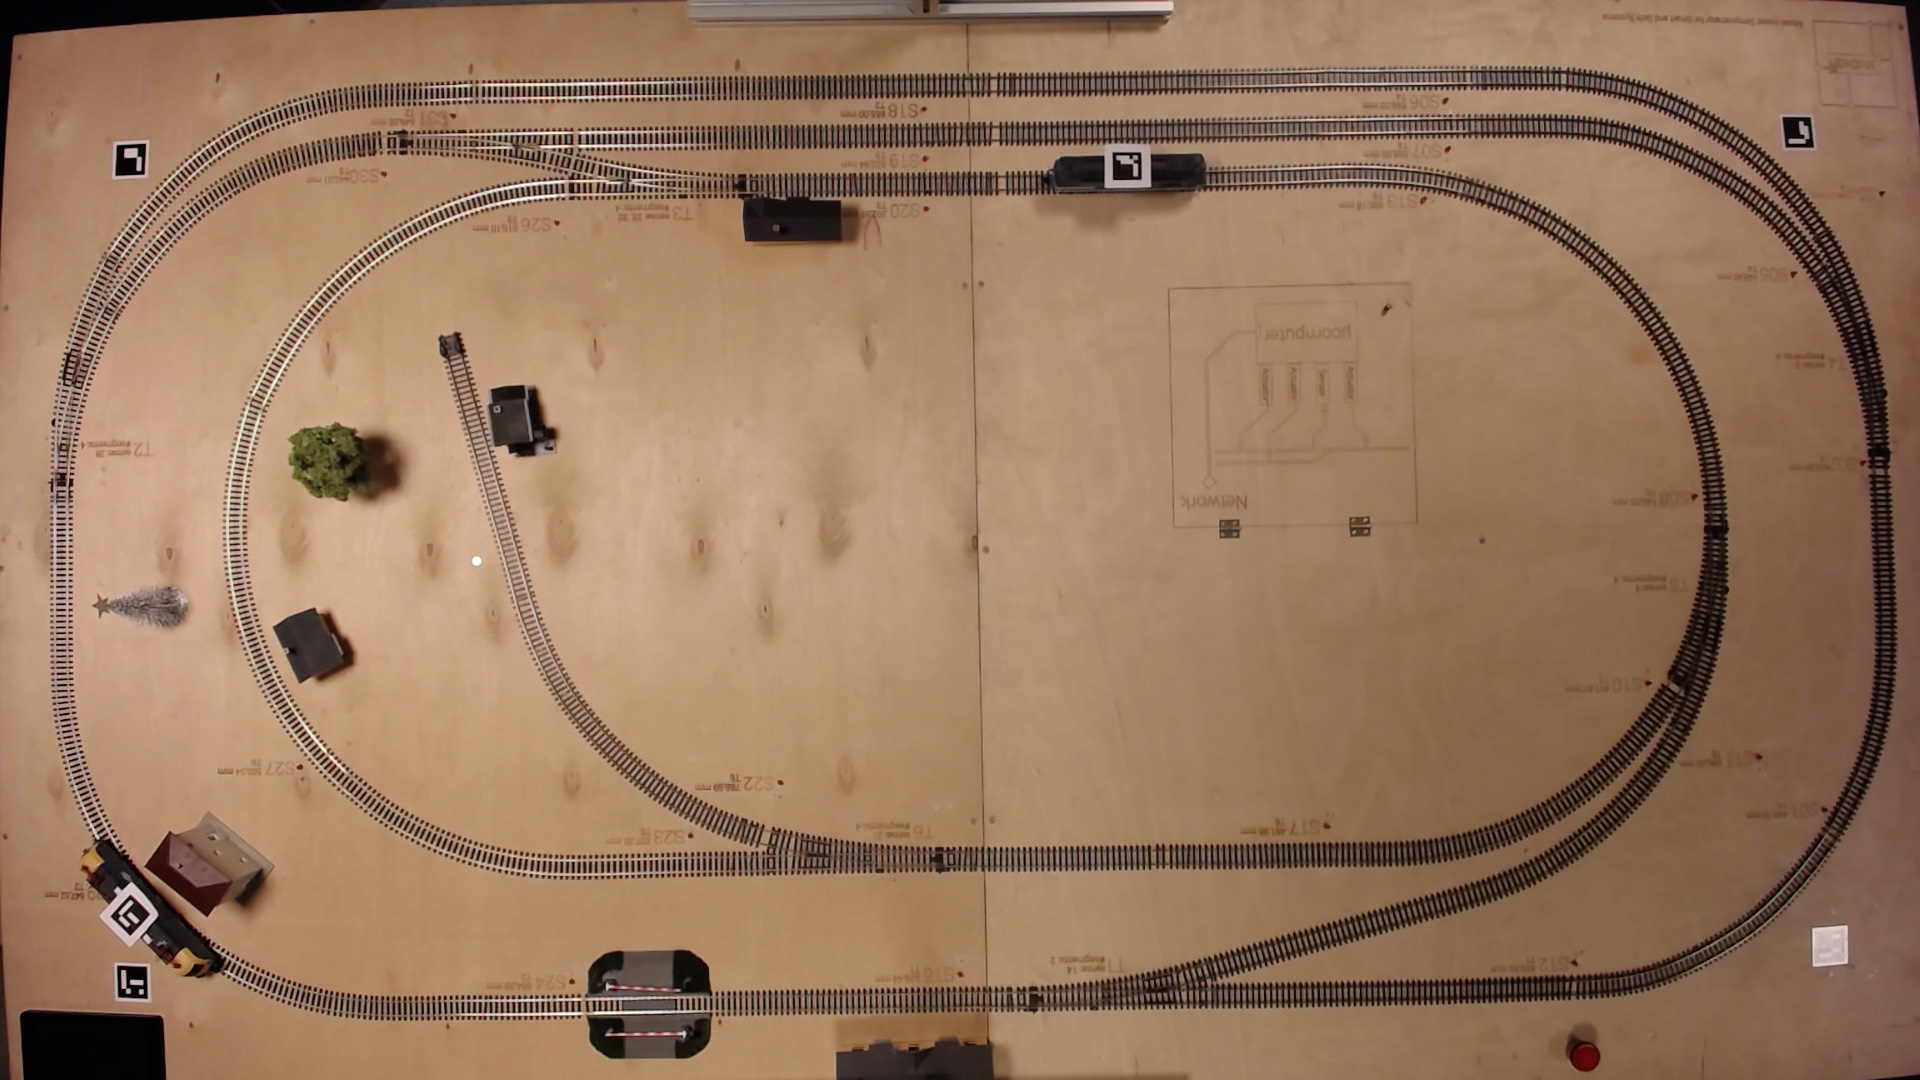
\includegraphics[width=150mm]{figures/modes3/overview.jpg}
	\caption{Railway system overview}
	\label{fig:overview}
\end{figure}
\section{Railway system basic components}
First of all I want to introduce the physical components and the basic process of the railway systems stub. There are 31 sections, with one blind track and 7 turnouts. The \ref{fig:layout} figure shows the layout of the railway elements with corresponding ids.
\begin{figure}[!ht]
	\centering
	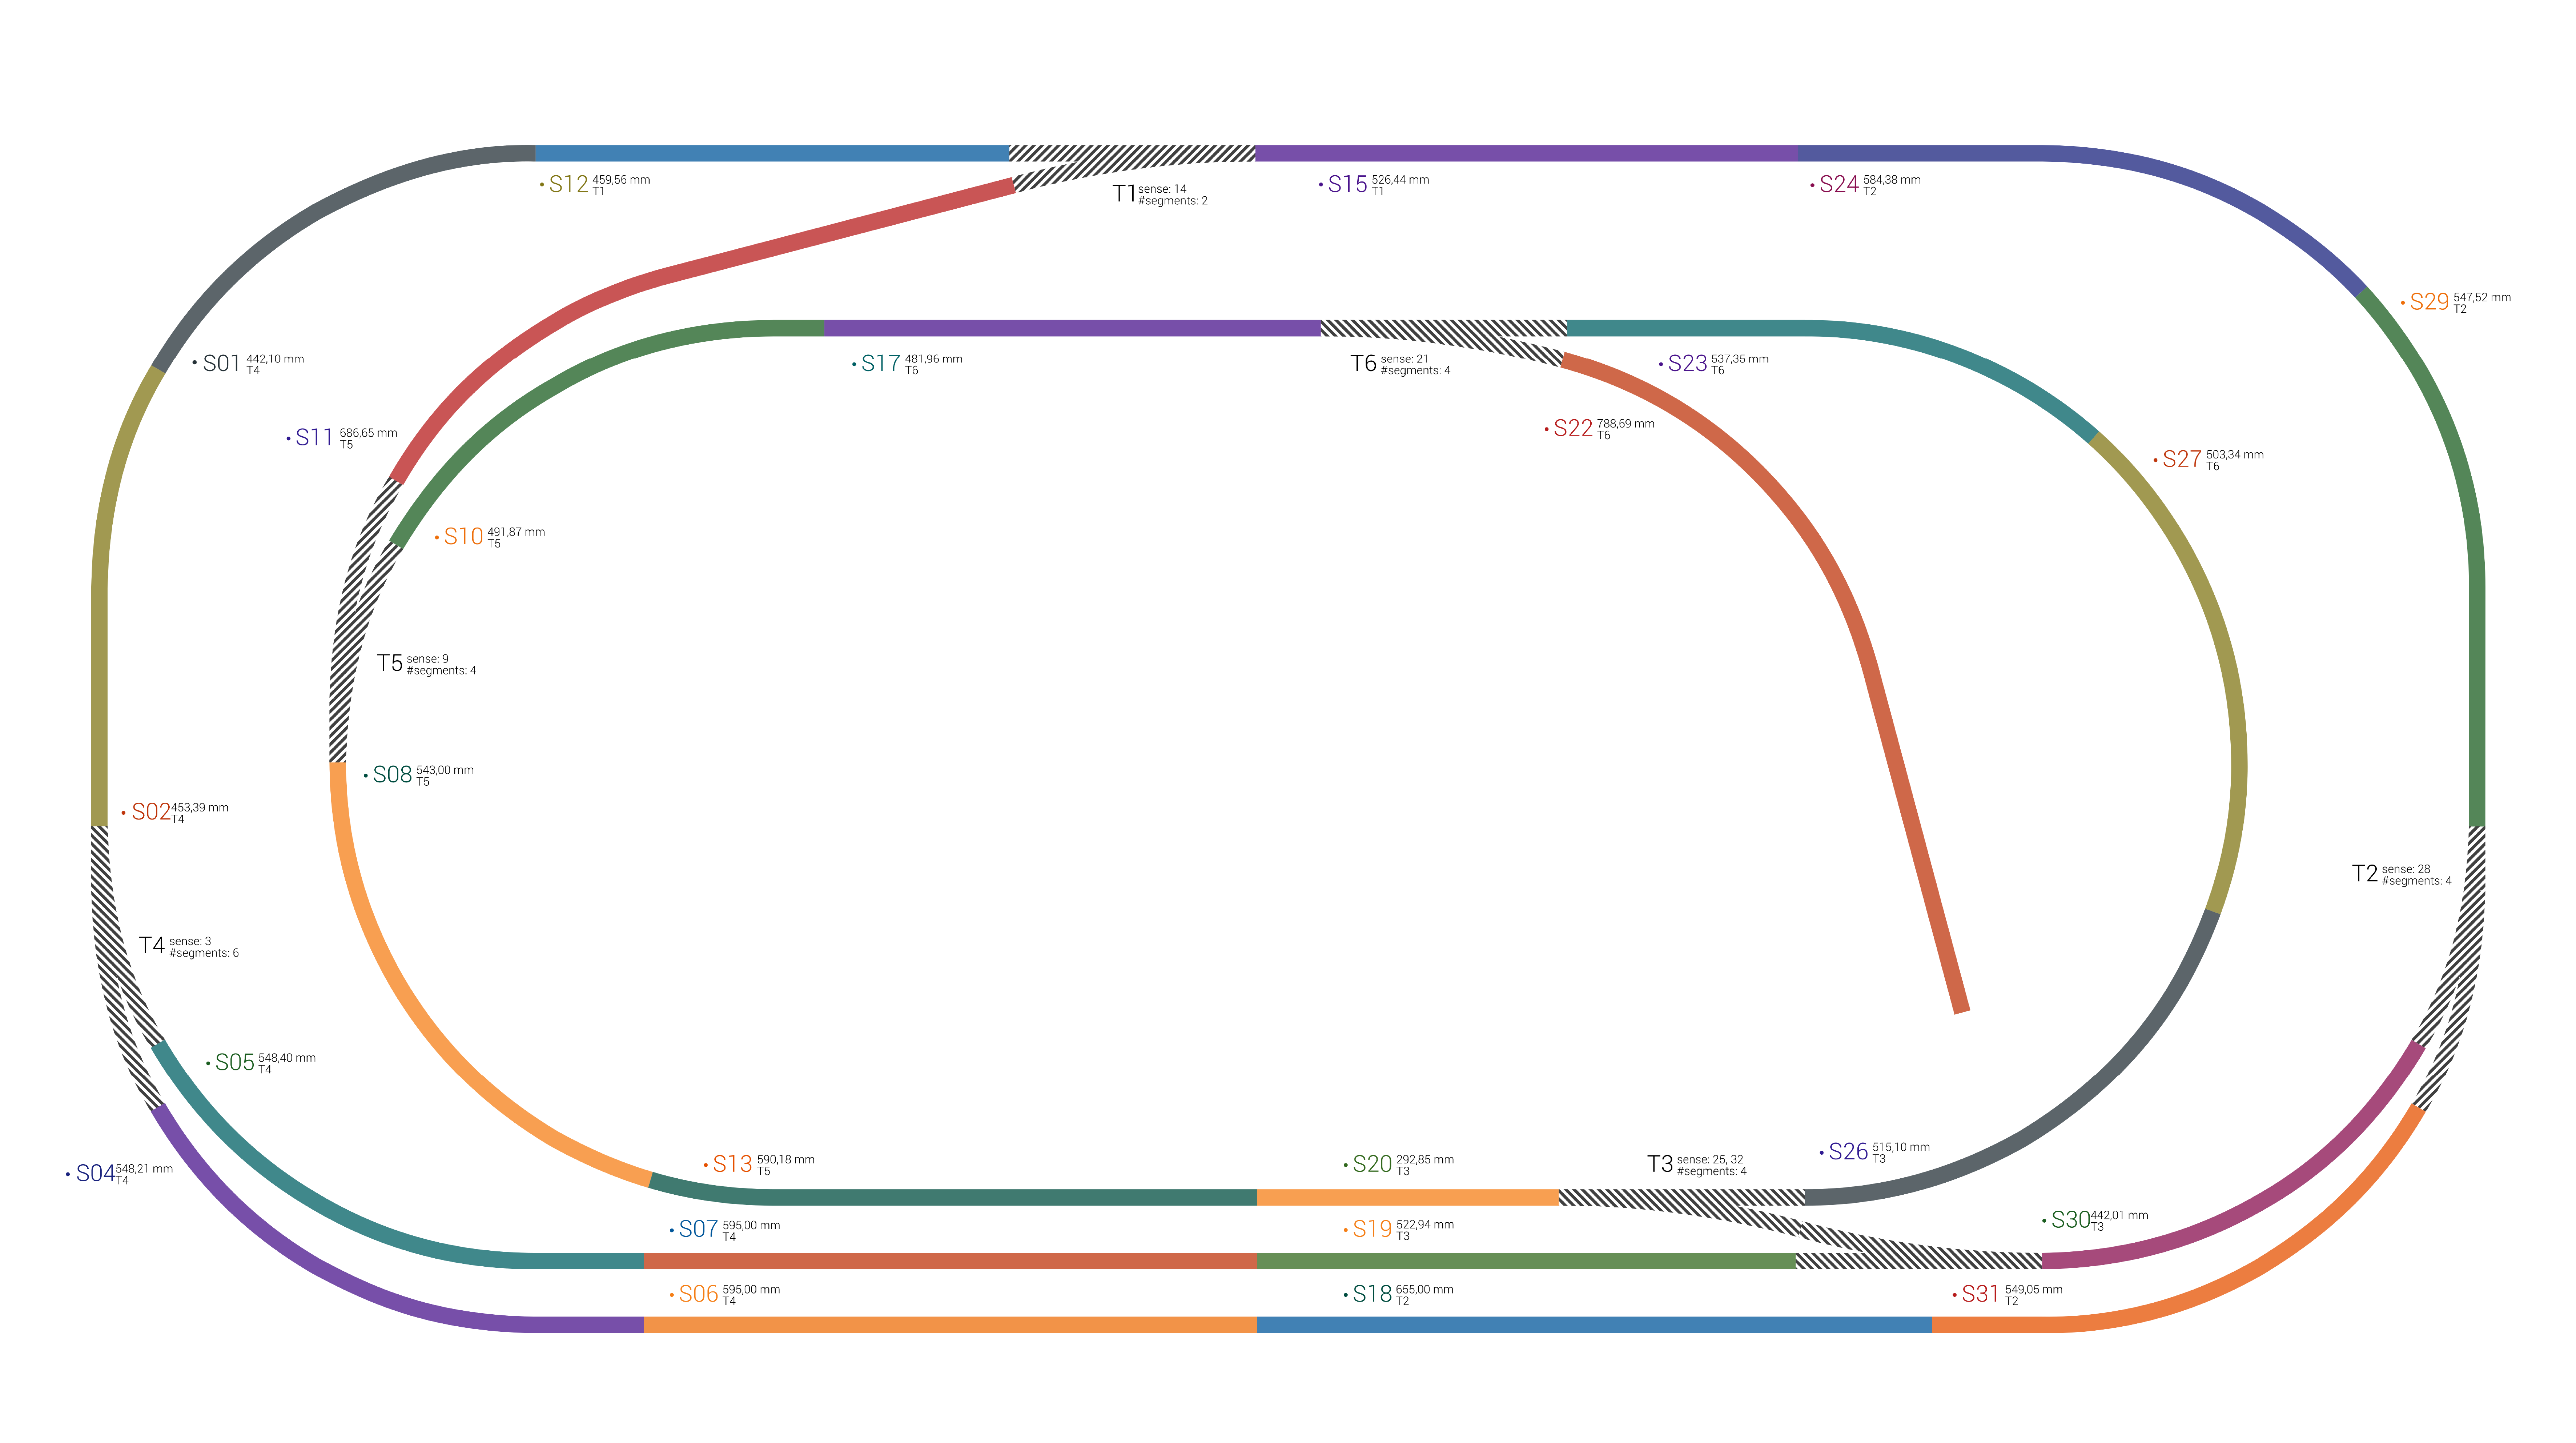
\includegraphics[width=150mm, keepaspectratio]{figures/modes3/layout2.png}
	\caption{Railway layout}
	\label{fig:layout}
\end{figure}
\paragraph{Section} 
First principal  element is a 15-20 cm long railway and connects to other 2 sections. Additionally each of them is connected to a command station, which gives them sufficient power source for moving the trains on them. In the figure \ref{fig:layout} these sections are identified by SXX strings, where XX is 2 unique digits and determines which bit shows this section's occupancy in the occupancy vector (see section \ref{section:OccupancyDetection} for more information). Each section lengths and responsible BeagleBone Black id are shown.
%\begin{figure}[!ht]
%	\centering
%	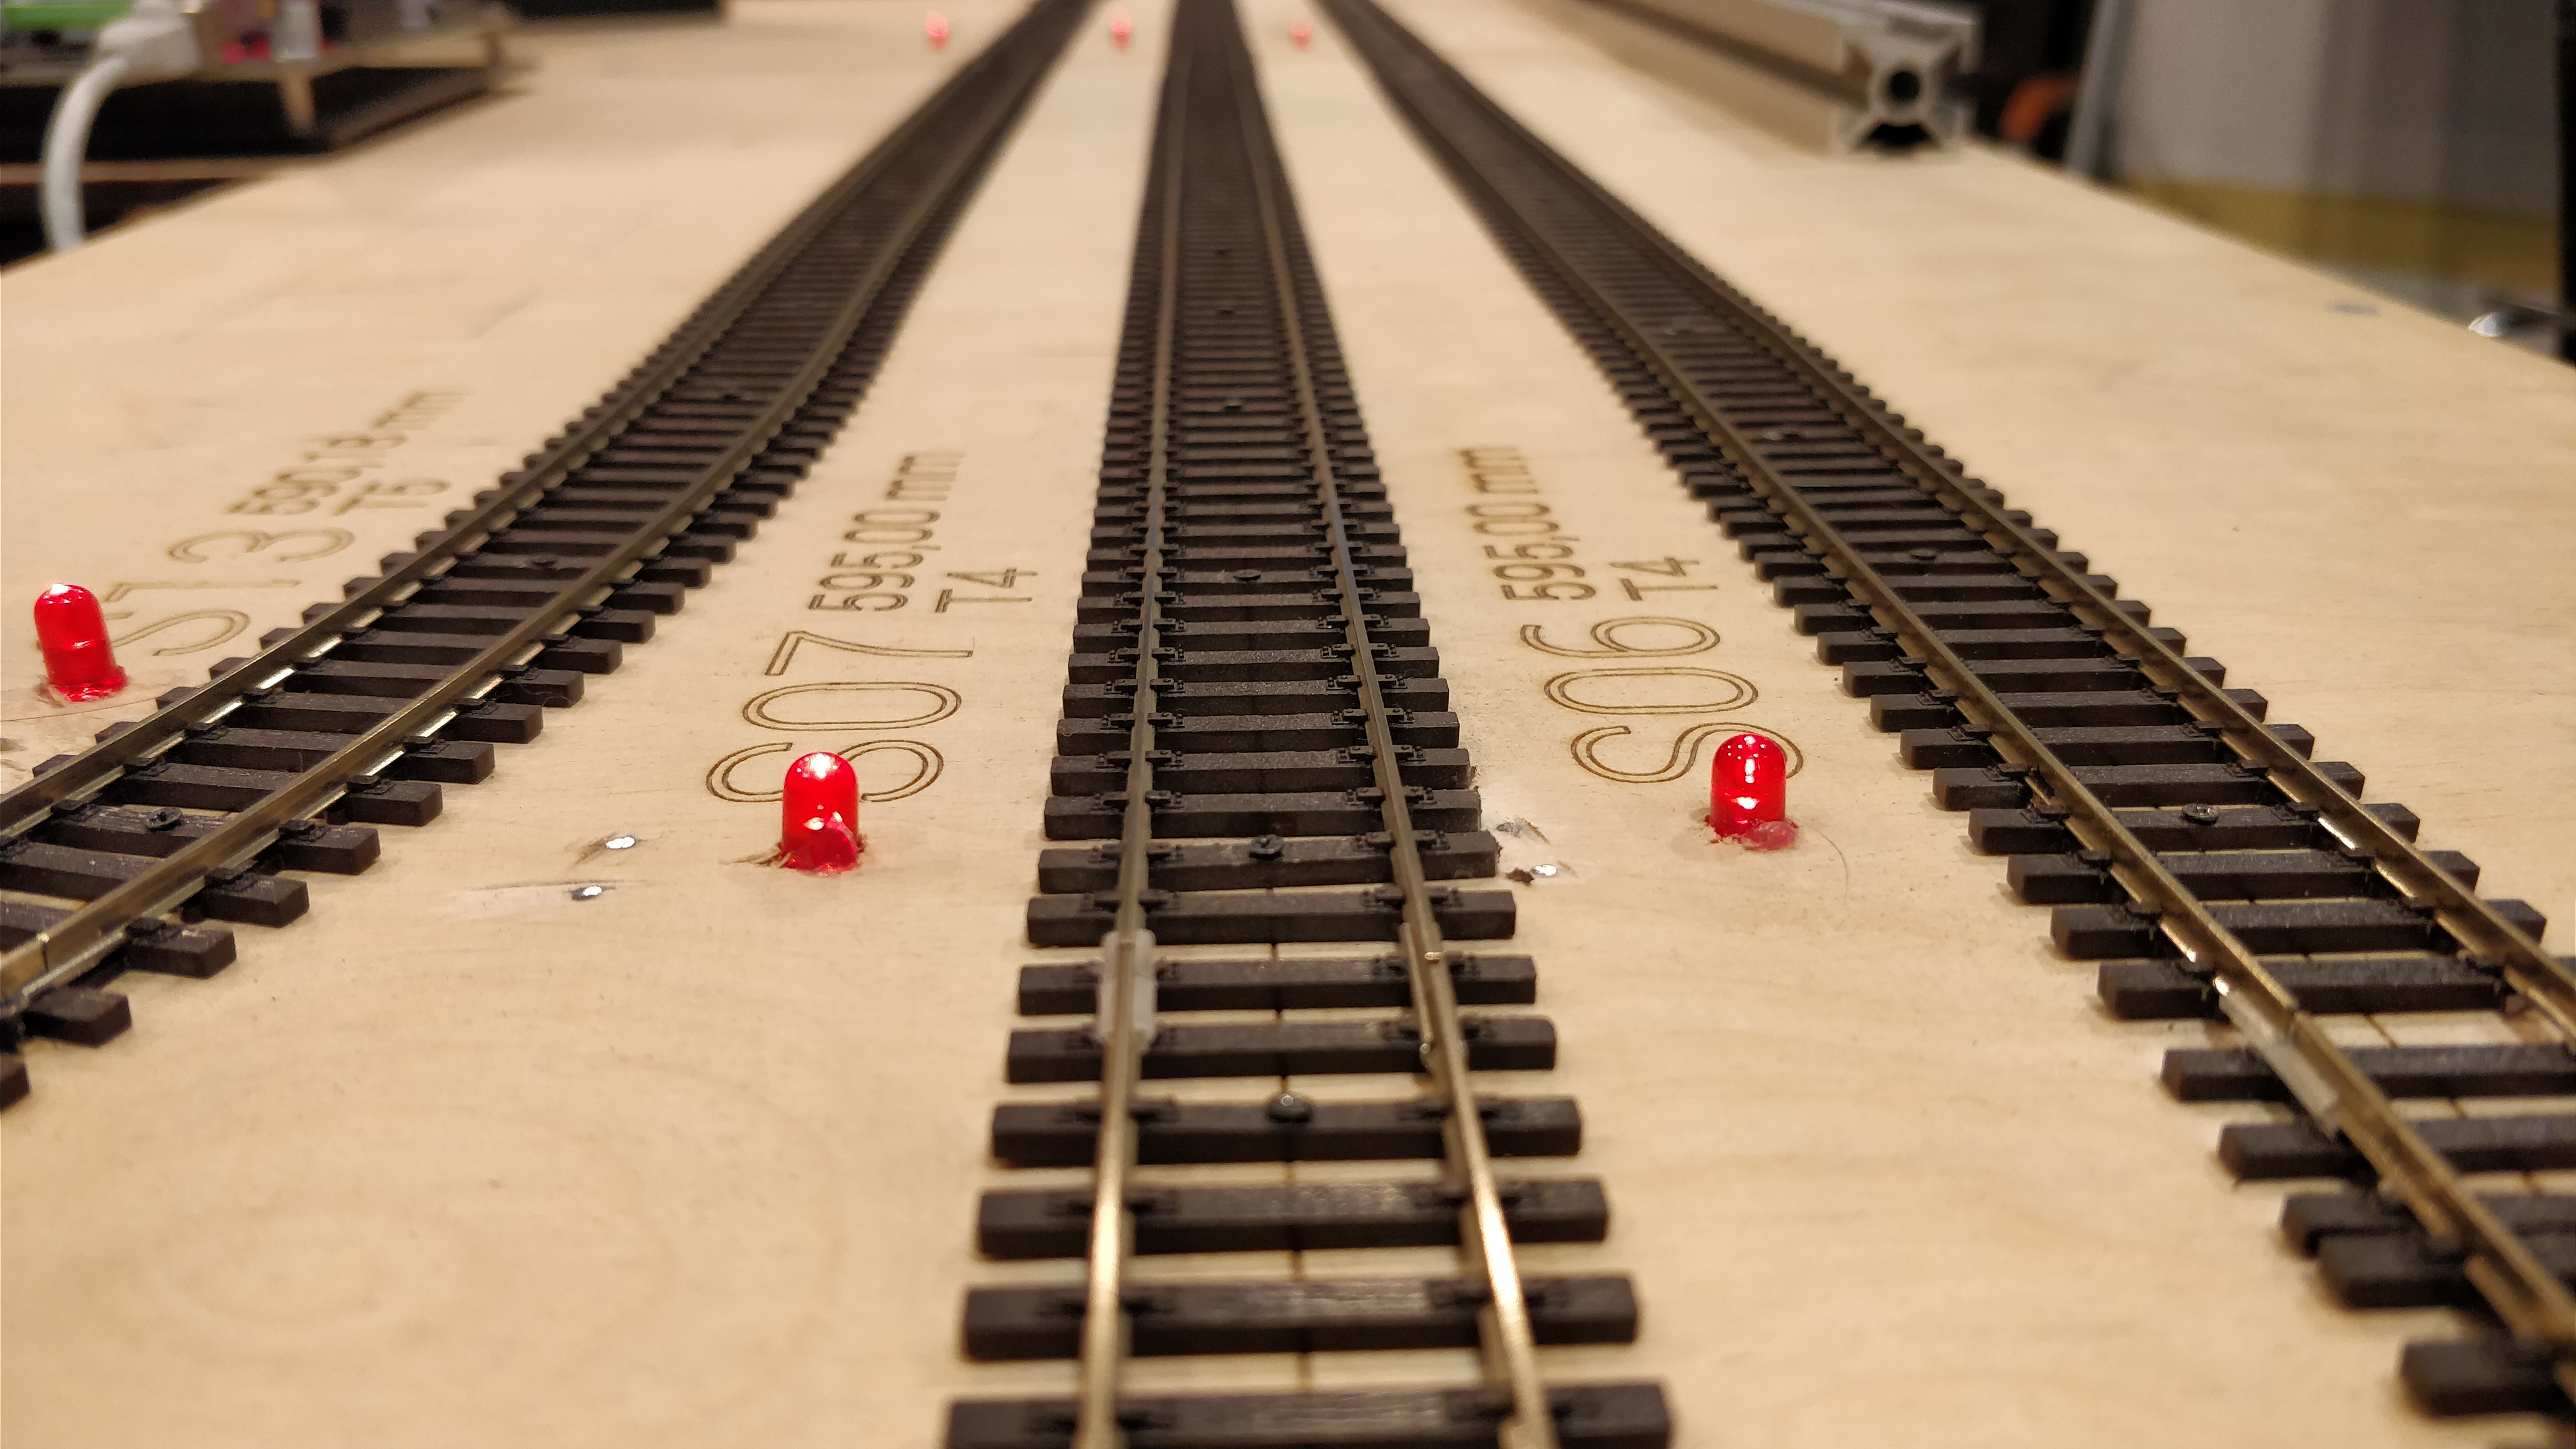
\includegraphics[width=150mm, keepaspectratio]{figures/modes3/section.jpg}
%	\caption{Railway Section}
%	\label{fig:section}
%\end{figure}
\paragraph{Turnout}
Second principal element, which can differentiate 2 paths as it can be seen on figure \ref{fig:turnoutDir}. Consequently the train which is going through one turnout can reach different sections depending on the state of the turnout. In the previous figure \ref{fig:layout} each turnout is visible as grey dashed section areas with turnout ID, sense (its value shows, which bit identifies this turnout's occupancy in the occupancy vector) and \textit{\#segments} as number of supervised sections by the BeagleBone Black. (see section \ref{section:OccupancyDetection} for more information) Each turnout id starts with T and ends with a numeric (1..6). 
\begin{figure}[!ht]
	\centering
	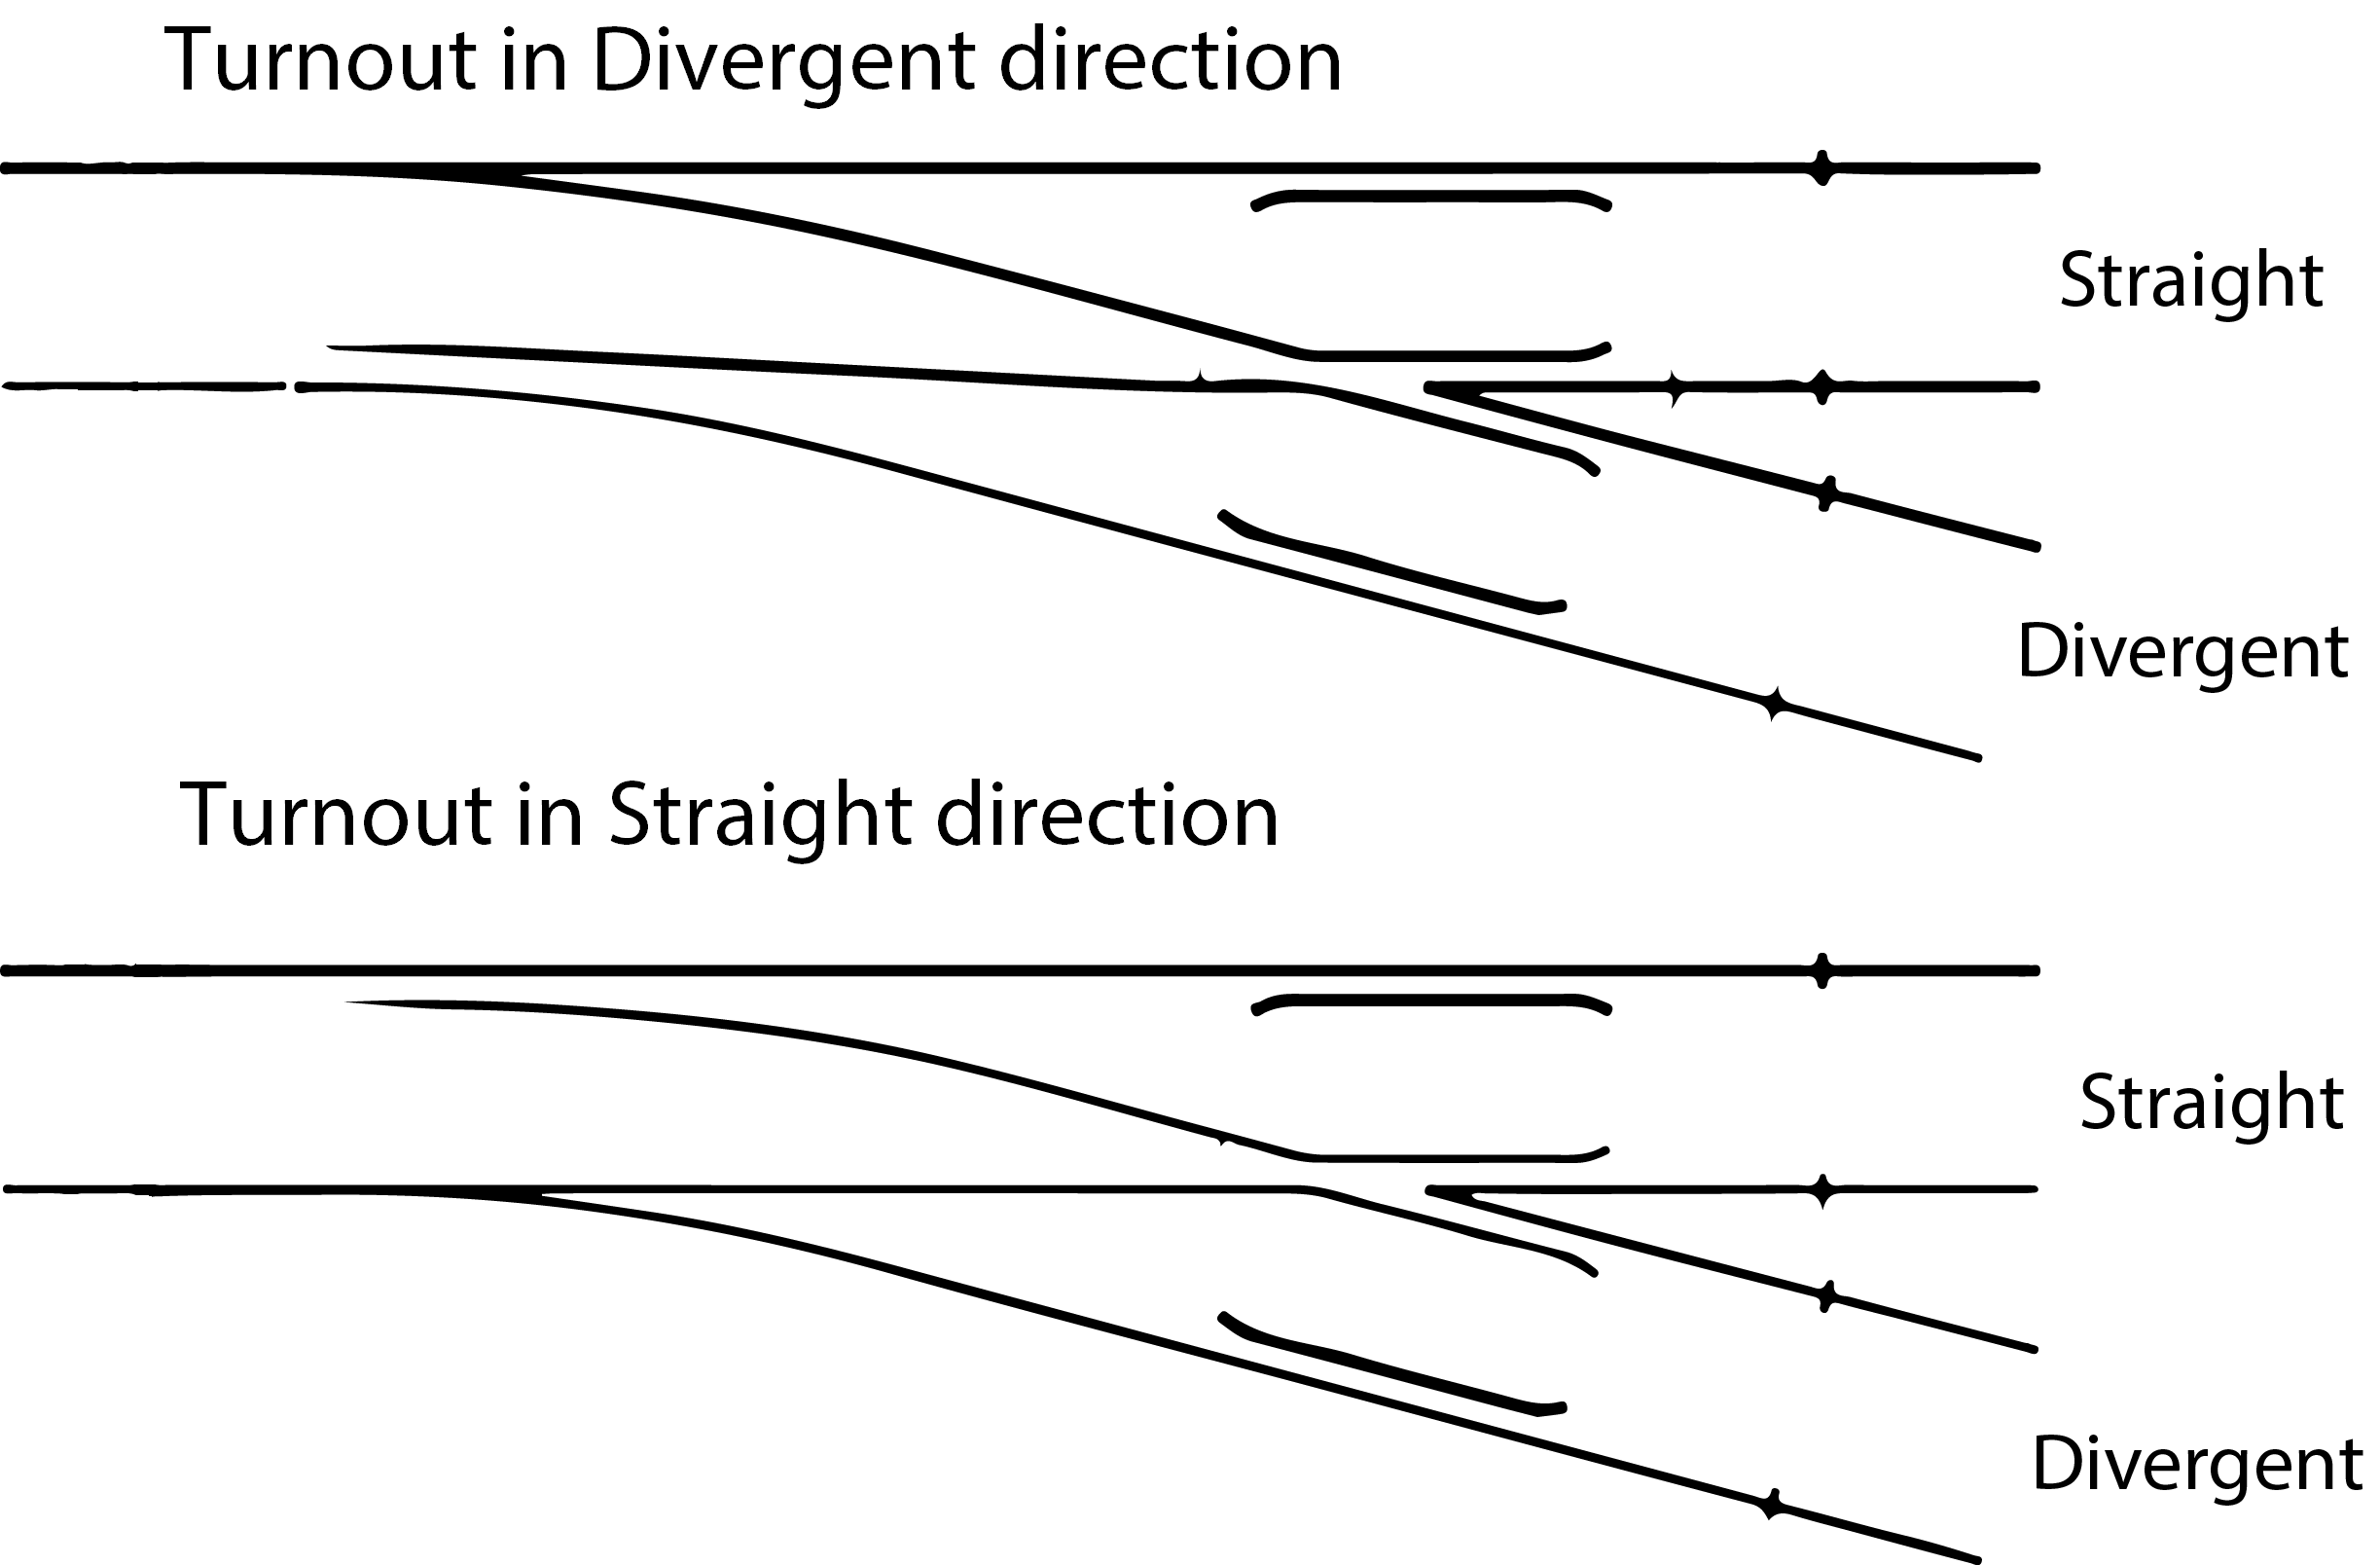
\includegraphics[width=150mm]{figures/modes3/turnout.png}
	\caption{Turnout directions}
	\label{fig:turnoutDir}
\end{figure}

\paragraph{Train}
There are 2 model trains, which can move on the sections and turnouts. The safety critical criteria is to avoid a train collision on the track.
%\begin{figure}[!ht]
%	\centering
%	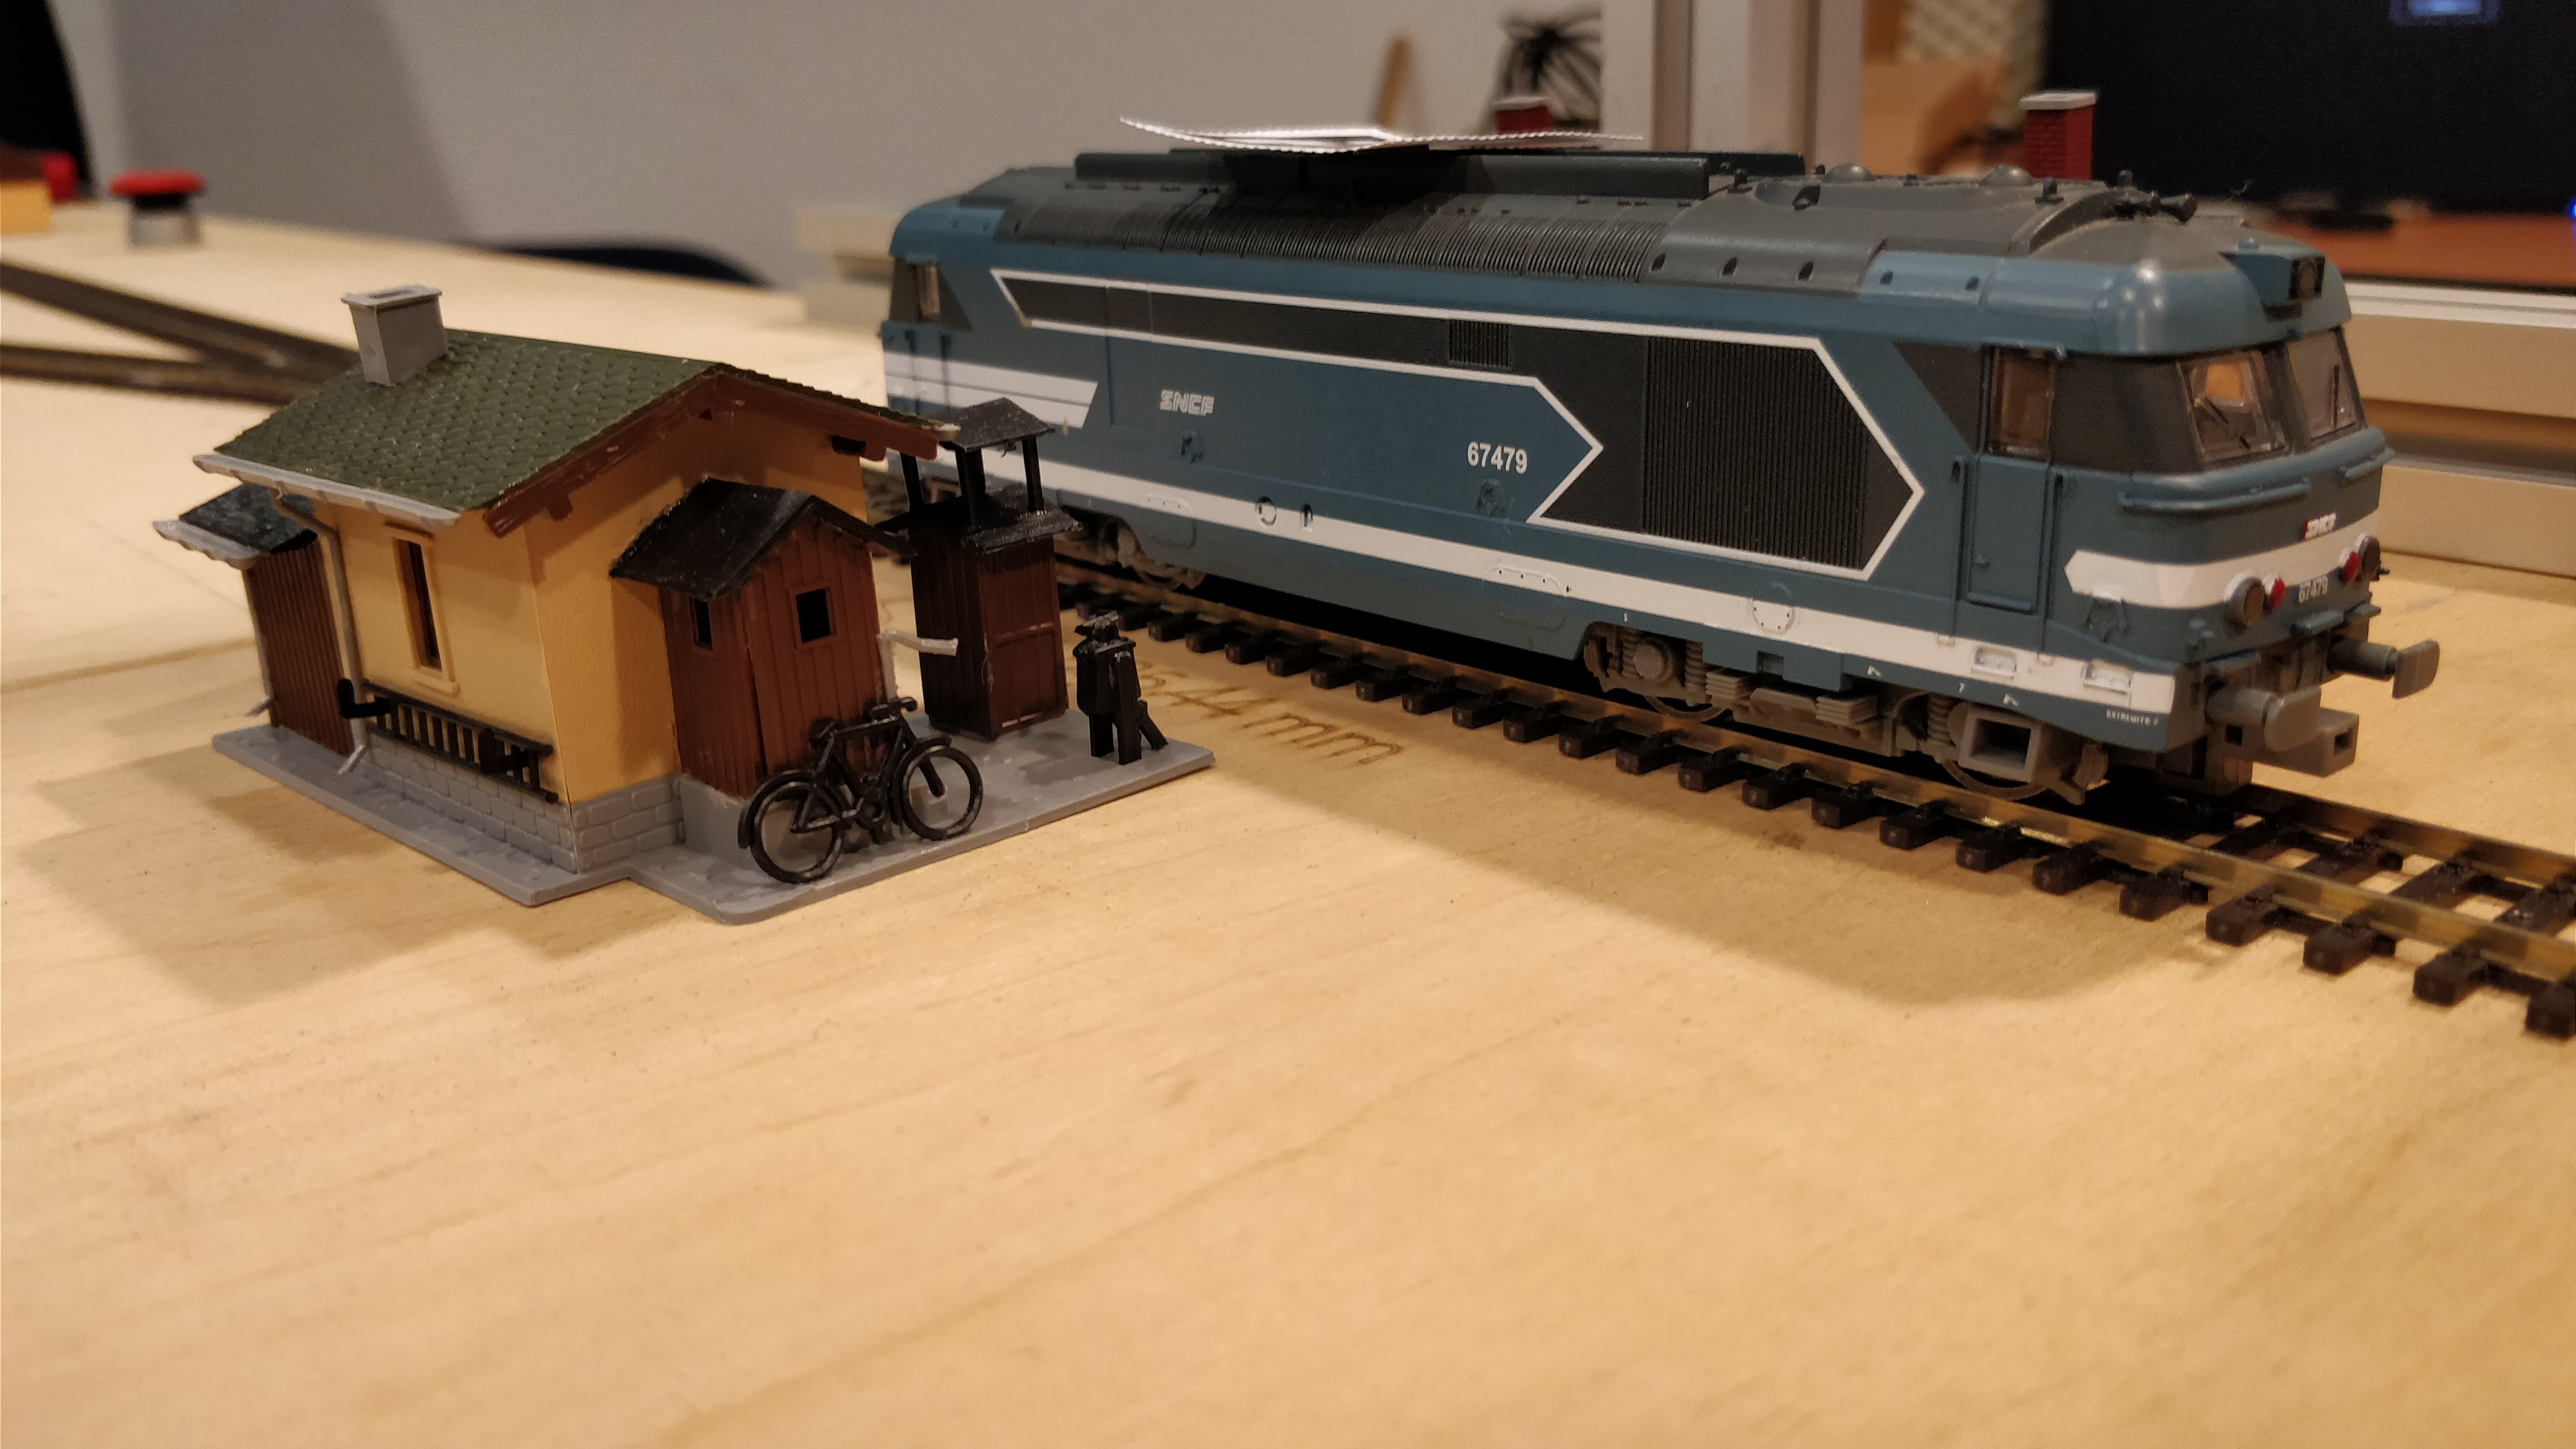
\includegraphics[width=150mm]{figures/modes3/train.jpg}
%	\caption{Train}
%	\label{fig:train}
%\end{figure}
\todo[inline]{ collision scenarios}


\paragraph{Command Station}
Supply power source for the sections which provides tension for the trains on the track.
\paragraph{Controller}
In connection with the \textit{Command Station} an XPressNet protocol \footnote{More details about XPressNet Protocol \url{http://www.lenzusa.com/1newsite1/Manuals/xpressnet.pdf}} based controller is attached to the system. This component's purpose is setting the direction and speed for each train on the track through the \textit{Command Station}

\section{Hardware extensions}
\subsection{Data processing units}
\todo[inline]{architecture digram  of BBB <-> HWs}

\paragraph{BeagleBone Black (BBB)}
An industrial microcontroller platform, which provides 4GB 8-bit eMMC on-board flash storage and 2x PRU 32-bit microcontrollers, which could satisfy the function for parallel monitoring. There are 6 BBB on the track connected to the railway, used for controlling and enable/disable each section.
% moved to the overall diagram%TODO add details about what is on the BBB
\paragraph{Rapsberry Pi 3}
A Rapsberry Pi microcontroller is dedicated to handle most of the software components related to the Railway demonstrator system. It has twice as large computing capacity in RAM and CPU as BBB.
\paragraph{Arduino}
Dedicated hardware element for reading from the 6 DigiSens-8-S88 output data through S88 protocol (see \ref{paragraph:SegmentSensor} section for details about the component). This communication layer requires proper timing conditions which the Arduino platform can satisfy.
\subsection{Custom hardware extensions}
\paragraph{BeagleBone Black cape and expanders}\label{paragraph:BBBcape}
The BeagleBone Black components expect 5VDC power source instead of 12VDC from our power supply. Because of that reason a so called cape have been created for each controller. Additionally the need for easy-to-use ports to attach additional circuits to the main board also have come up. The expanders could be used to extend the functionality of one BeagleBone unit, which is on the figure \ref{fig:cape}.
\begin{figure}[!ht]
	\centering
	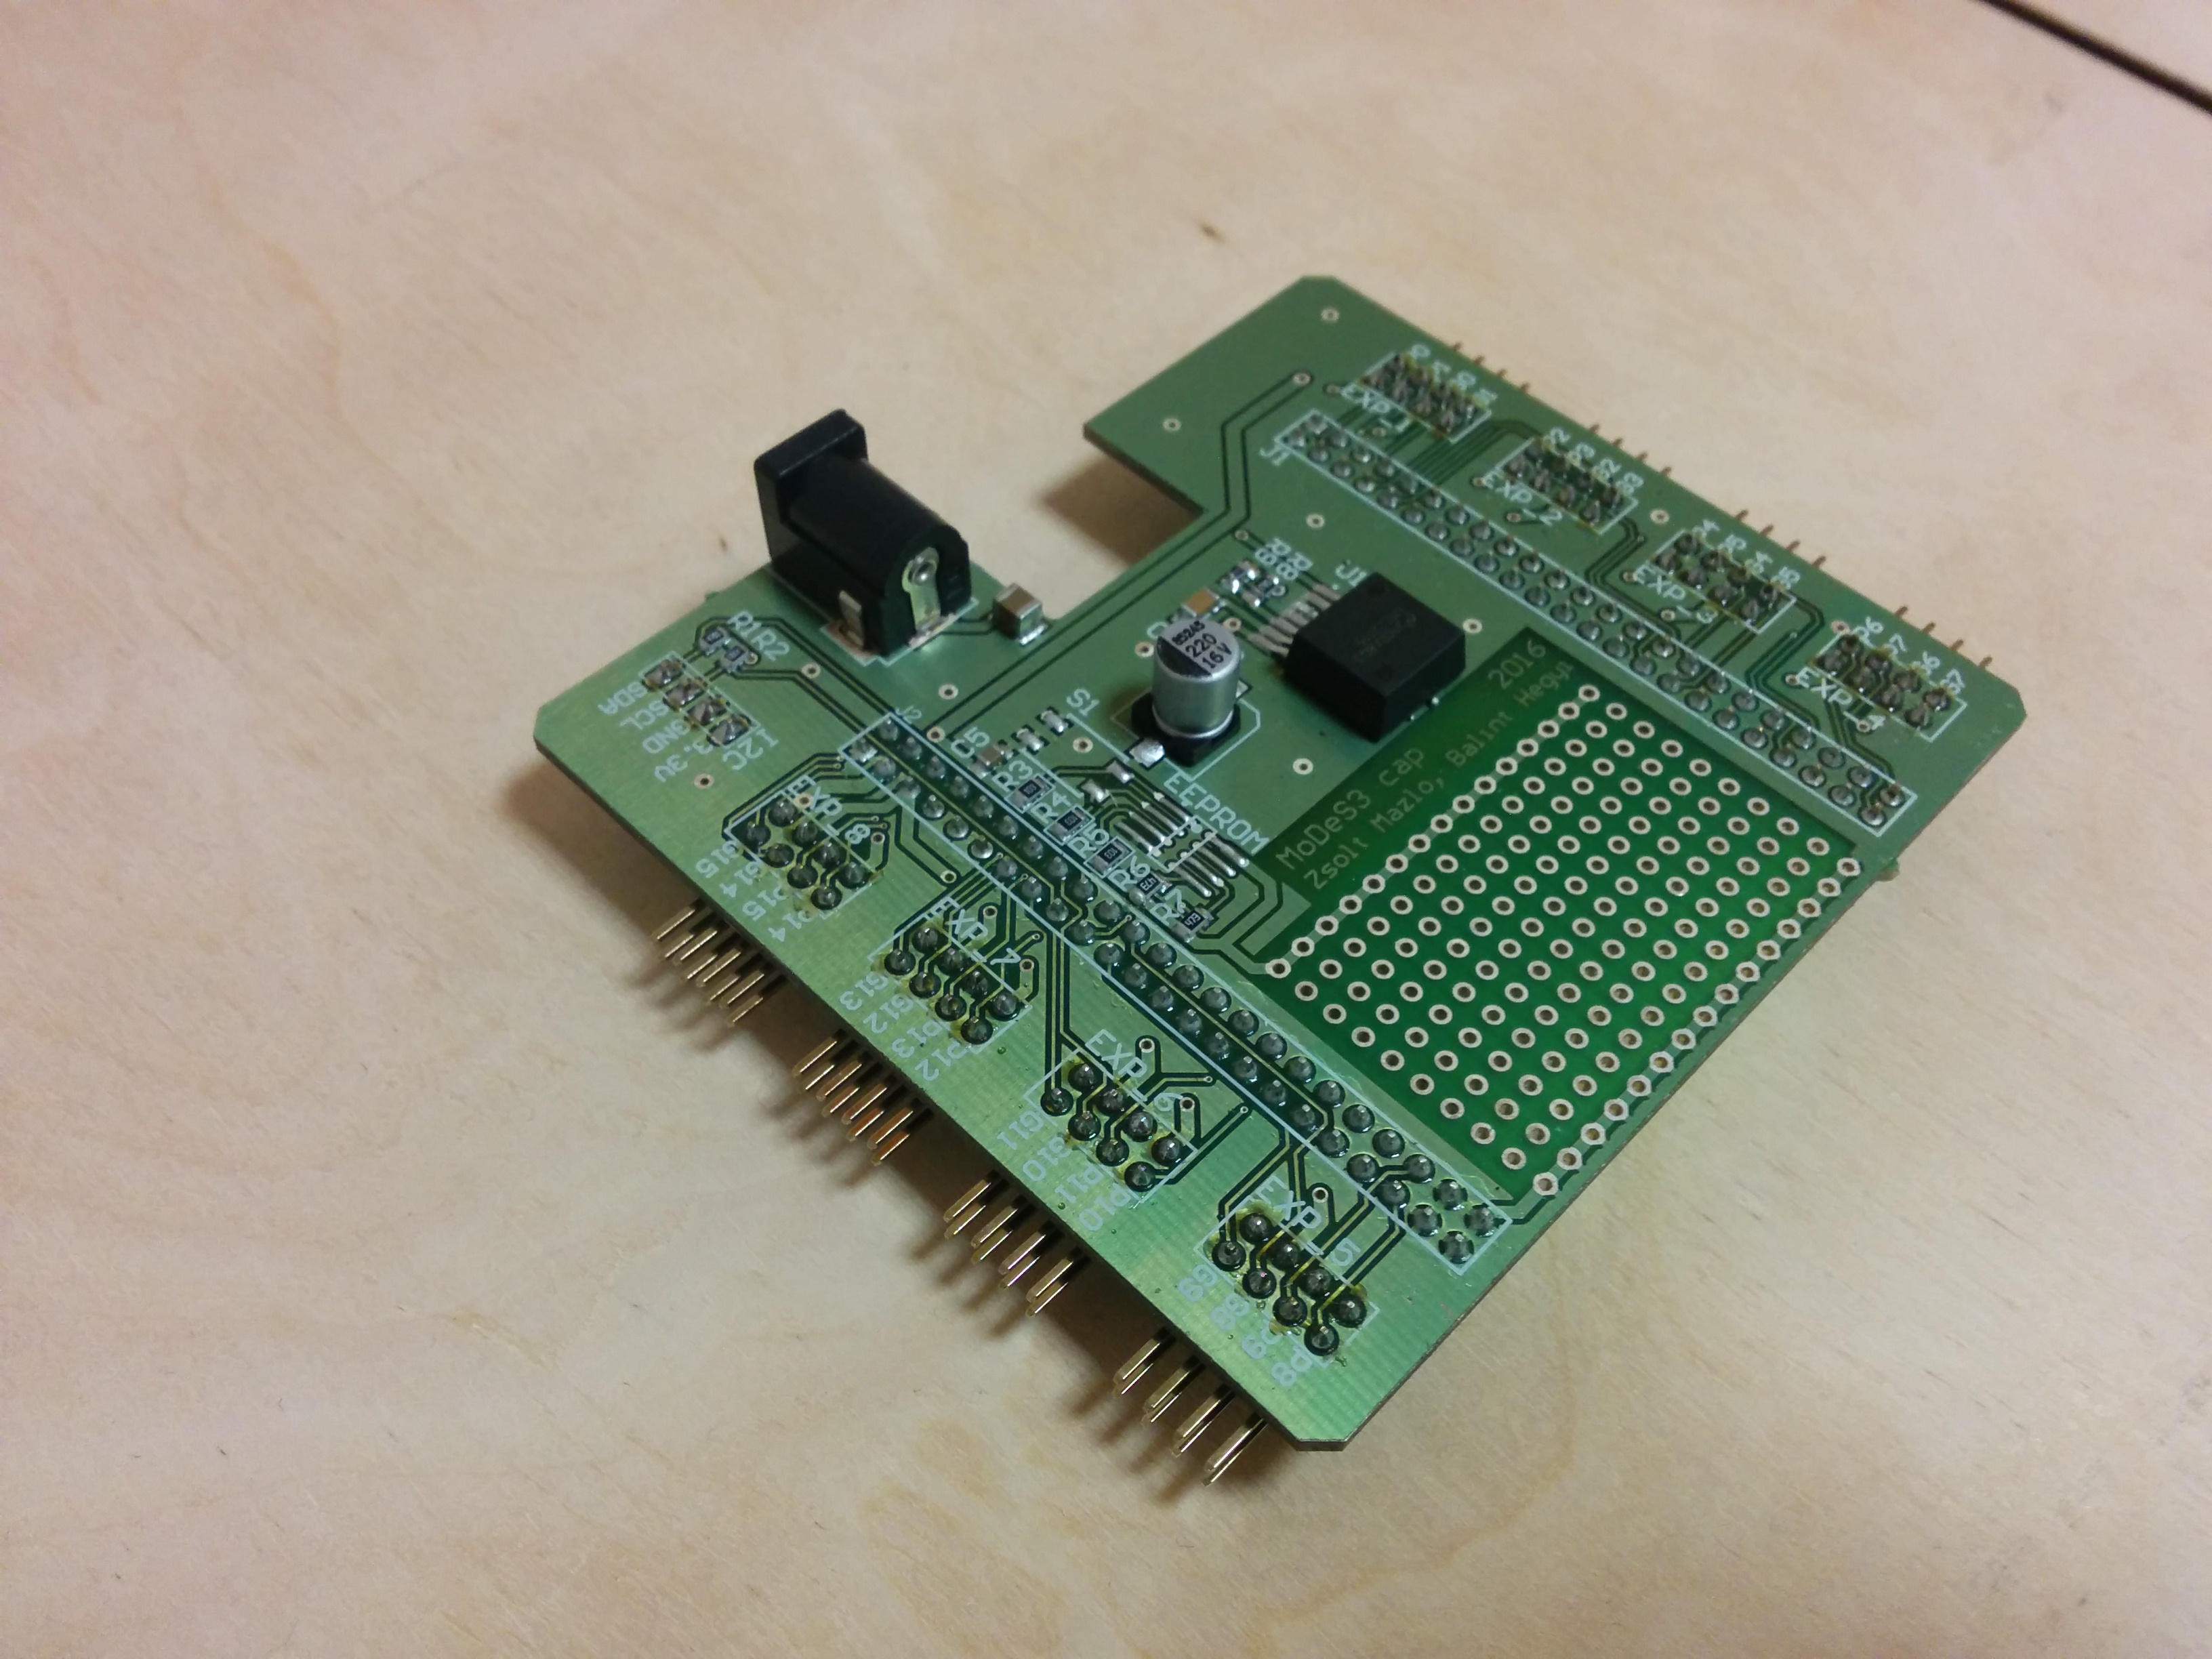
\includegraphics[width=150mm]{figures/modes3/cap1.jpg}
	\caption{Cape and expander for BeagleBone Black}
	\label{fig:cape}
\end{figure}

Each cape have 8 general purpose expander slot, for which the pin layout is expressed in the following \ref{table:expander_pin_layout} table.

\begin{table}
	\caption{Pin layout}
	\label{table:expander_pin_layout}
	\begin{center}
		\renewcommand{\arraystretch}{1.8}
		\begin{tabu} to 0.3\textwidth { | X[c] | X[c] | X[c] | X[c] |}
			\hline
			G3 & G2 & G1 & G0 \\
			\hline
			3V3  & 5V  & Gnd  & 12V\\
			\hline
		\end{tabu}
	\end{center}
\end{table} 

The upper row of each connector is dedicated for GPIO connections. Two of the GPIO pins connected to the application processor (labeled with G0..G15), and the remaining two GPIO pins are connected to the PRU unit (labeled P0..P15).

With this setup, the PRU and the application processor can cooperate on hardware level. Also, if we want we could use the P0..P15 GPIOs from the application processor as well.

\paragraph{Segment sensor}\label{paragraph:SegmentSensor}
 The DigiSens-8-S88 component is an off-the-shelf product, which can detect the occupancy for 8 sections.\footnote{More information about the product can be found here:\url{http://www.digitools.hu/termekek/erzekelok/digisens-8-s88}}.

\paragraph{Segment actuator}
Segment Actuator expanders are designed to stop a train on the corresponding segment. The concept behind this expander based on the Lenz Asymmetrical DCC and ABC functionality of train-decoders. \footnote{The following descriptions are based on \url{https://tonystrains.com/lenz-asymmetrical-dcc-and-abc/} article.}

\begin{figure}[!ht]
	\centering
	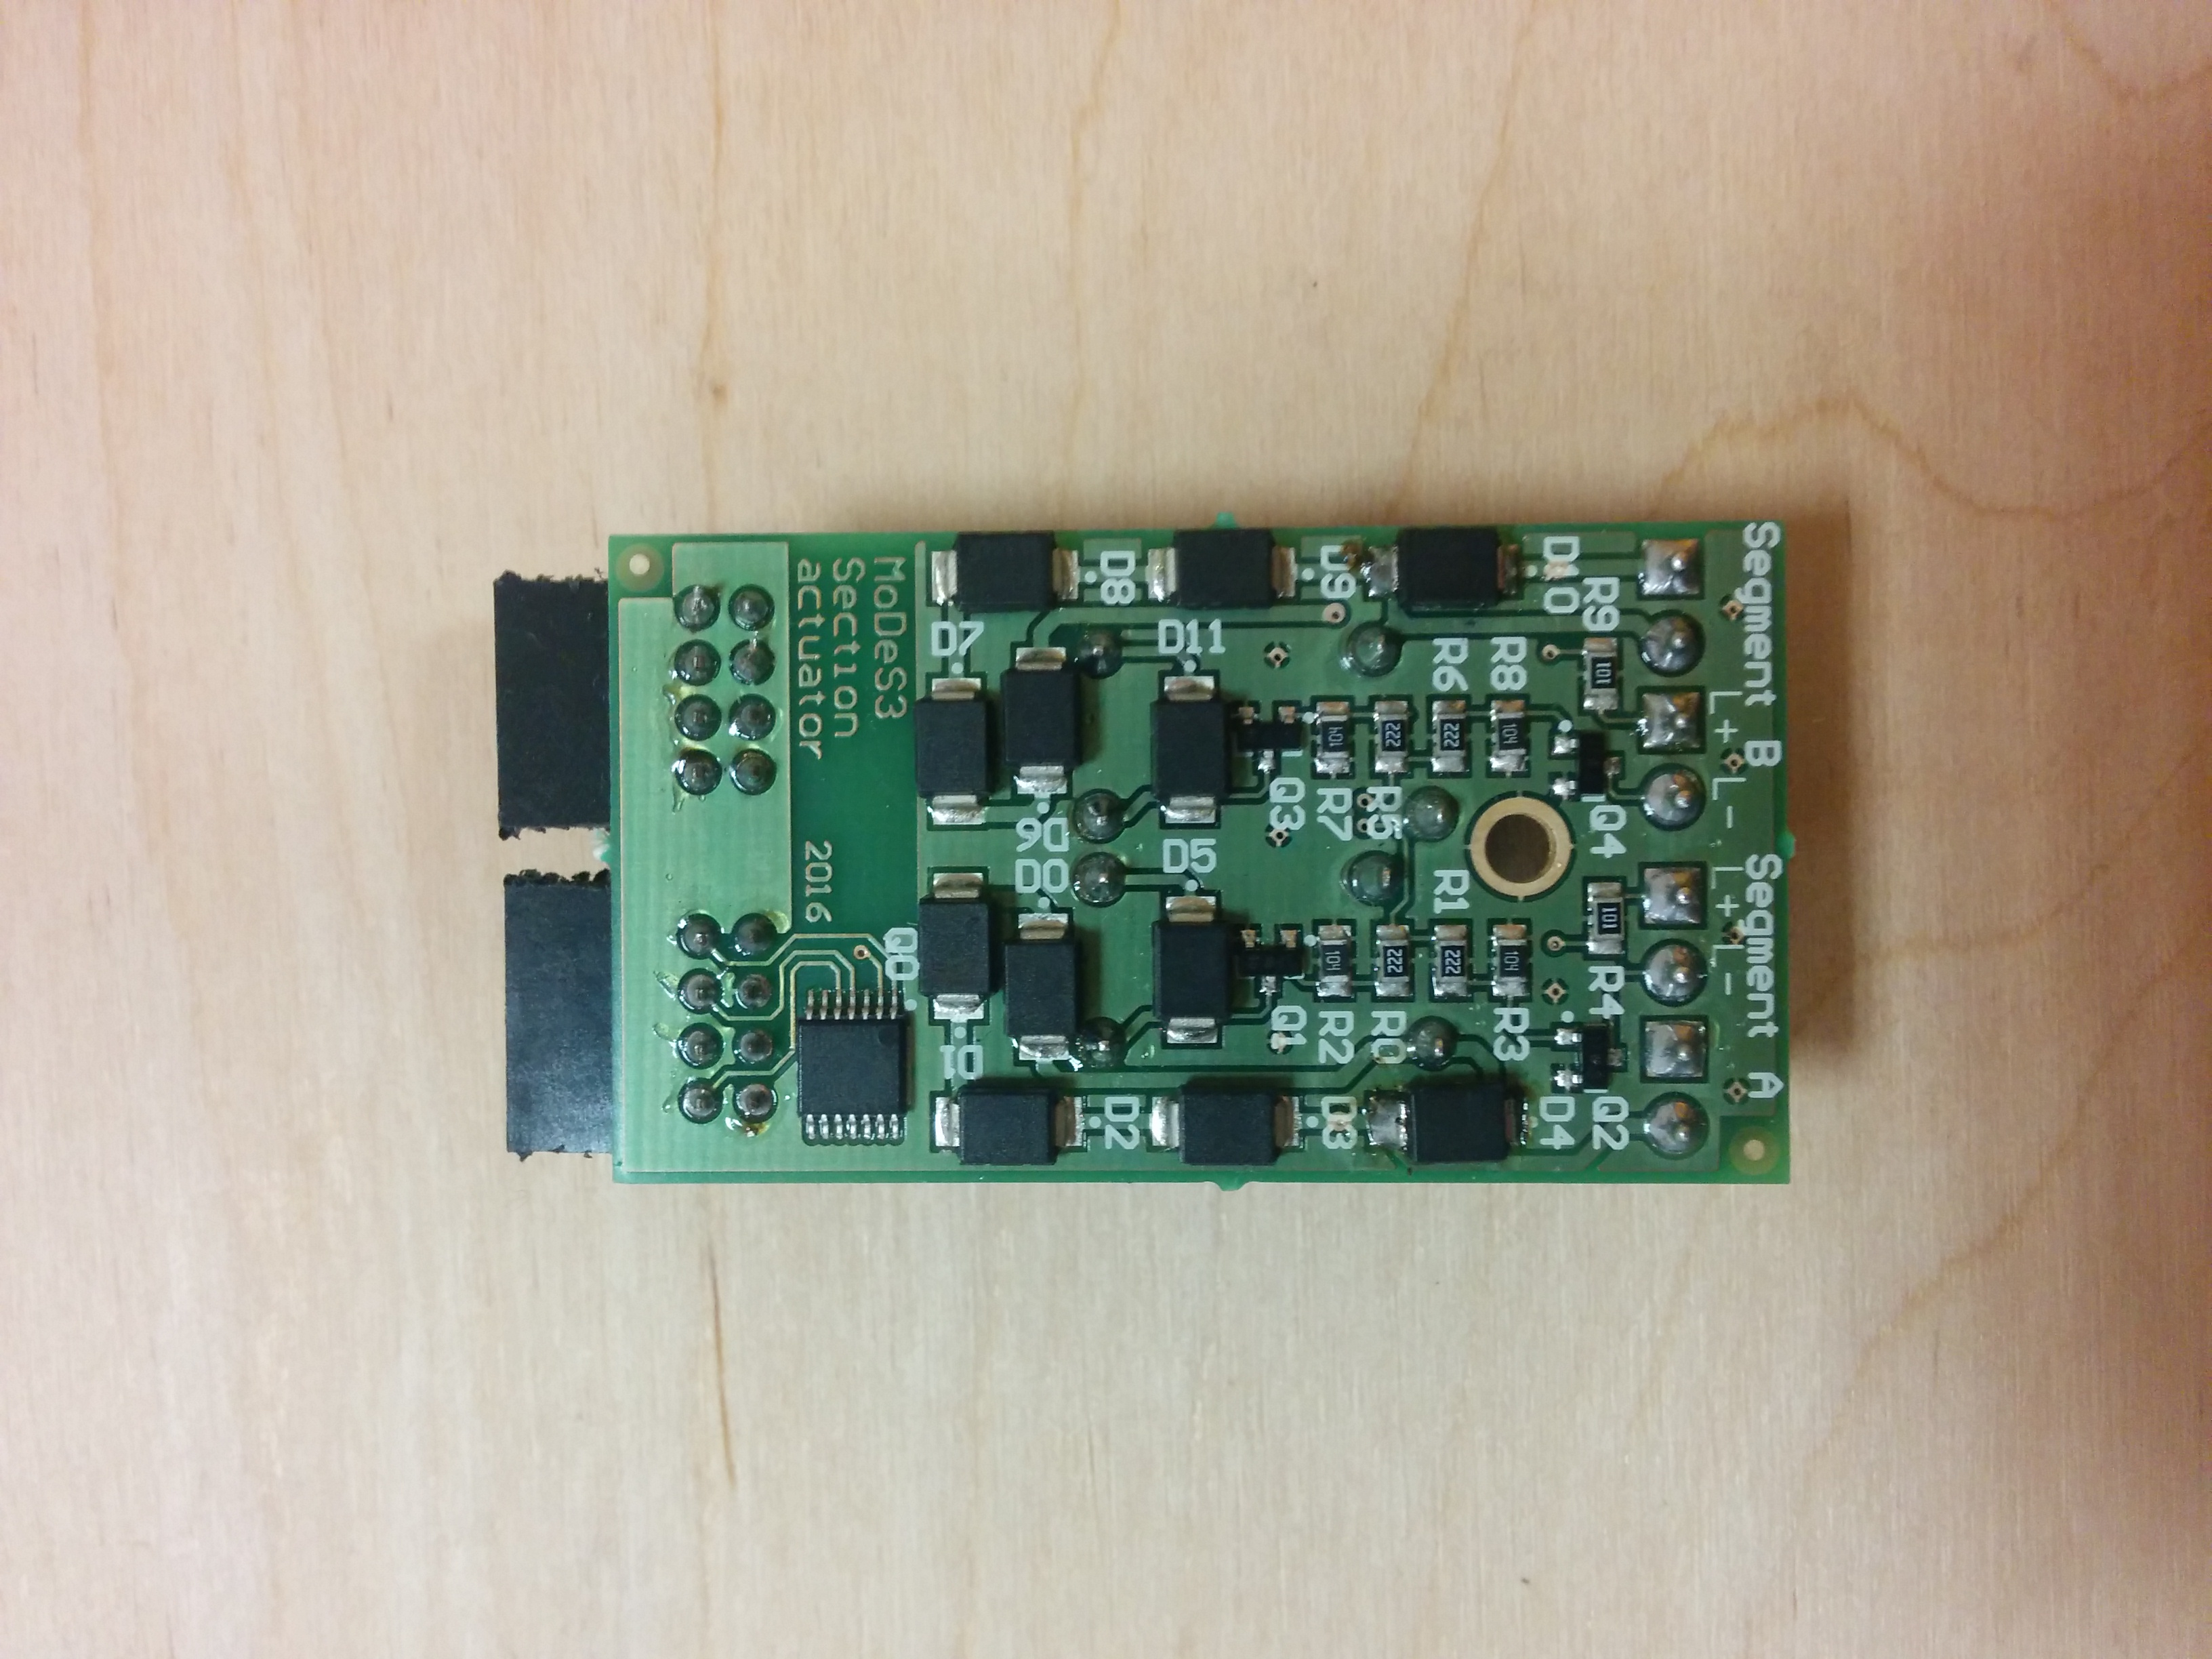
\includegraphics[width=100mm]{figures/modes3/segment-top.jpg}
	\caption{Segment actuator top view}
	\label{fig:segmentTop}
\end{figure}

ABC (Automatic Brake Control) works in conjunction with Asymmetrical DCC. Asymmetrical DCC is a way to trigger ABC in the decoder. This gives the ability to stop trains at a section of the track with Asymmetrical DCC.

\begin{figure}[!ht]
	\centering
	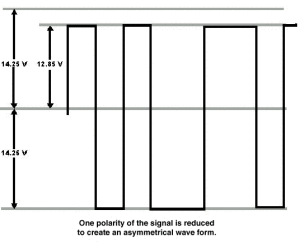
\includegraphics[width=100mm]{figures/modes3/DCC.png}
	\caption{Asymmetric DCC voltages}
	\label{fig:dcc}
\end{figure}

\todo[inline]{figure needed}
The Asymmetrical DCC signal is generated by offsetting one phase of the DCC signal. This signal then triggers the Automatic Brake Control in the decoder. This causes the engine to stop at the distance set up in the Constant Stopping Distance feature. We implemented this using five diodes. %connected in the form as shown in the figure below.

%\begin{figure}[!ht]
%	\centering
%	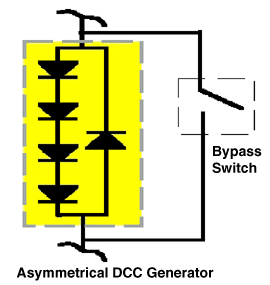
\includegraphics[width=50mm]{figures/modes3/abc.png}
%	\caption{Asymmetric DCC voltages}
%	\label{fig:abc}
%\end{figure}

The Segment Actuators uses this setup and also gives an interface (with GPIOs) to enable or disable this feature. Every Segment Actuator expander has two slots (A or B) and can enable or disable two segments. Each segment can be enabled setting two GPIOs to HIGH level, one connected to the PRU and one connected to the application processor.

\paragraph{Turnout actuator}
Turnout Actuator expanders can switch turnouts on the table between their states. Previously, we have managed to solve this with COTS units, but in that case we were not able to query the position of the switch programmatically. This expander gives the ability for both switching the turnout and sensing its state.

\begin{figure}[!ht]
	\centering
	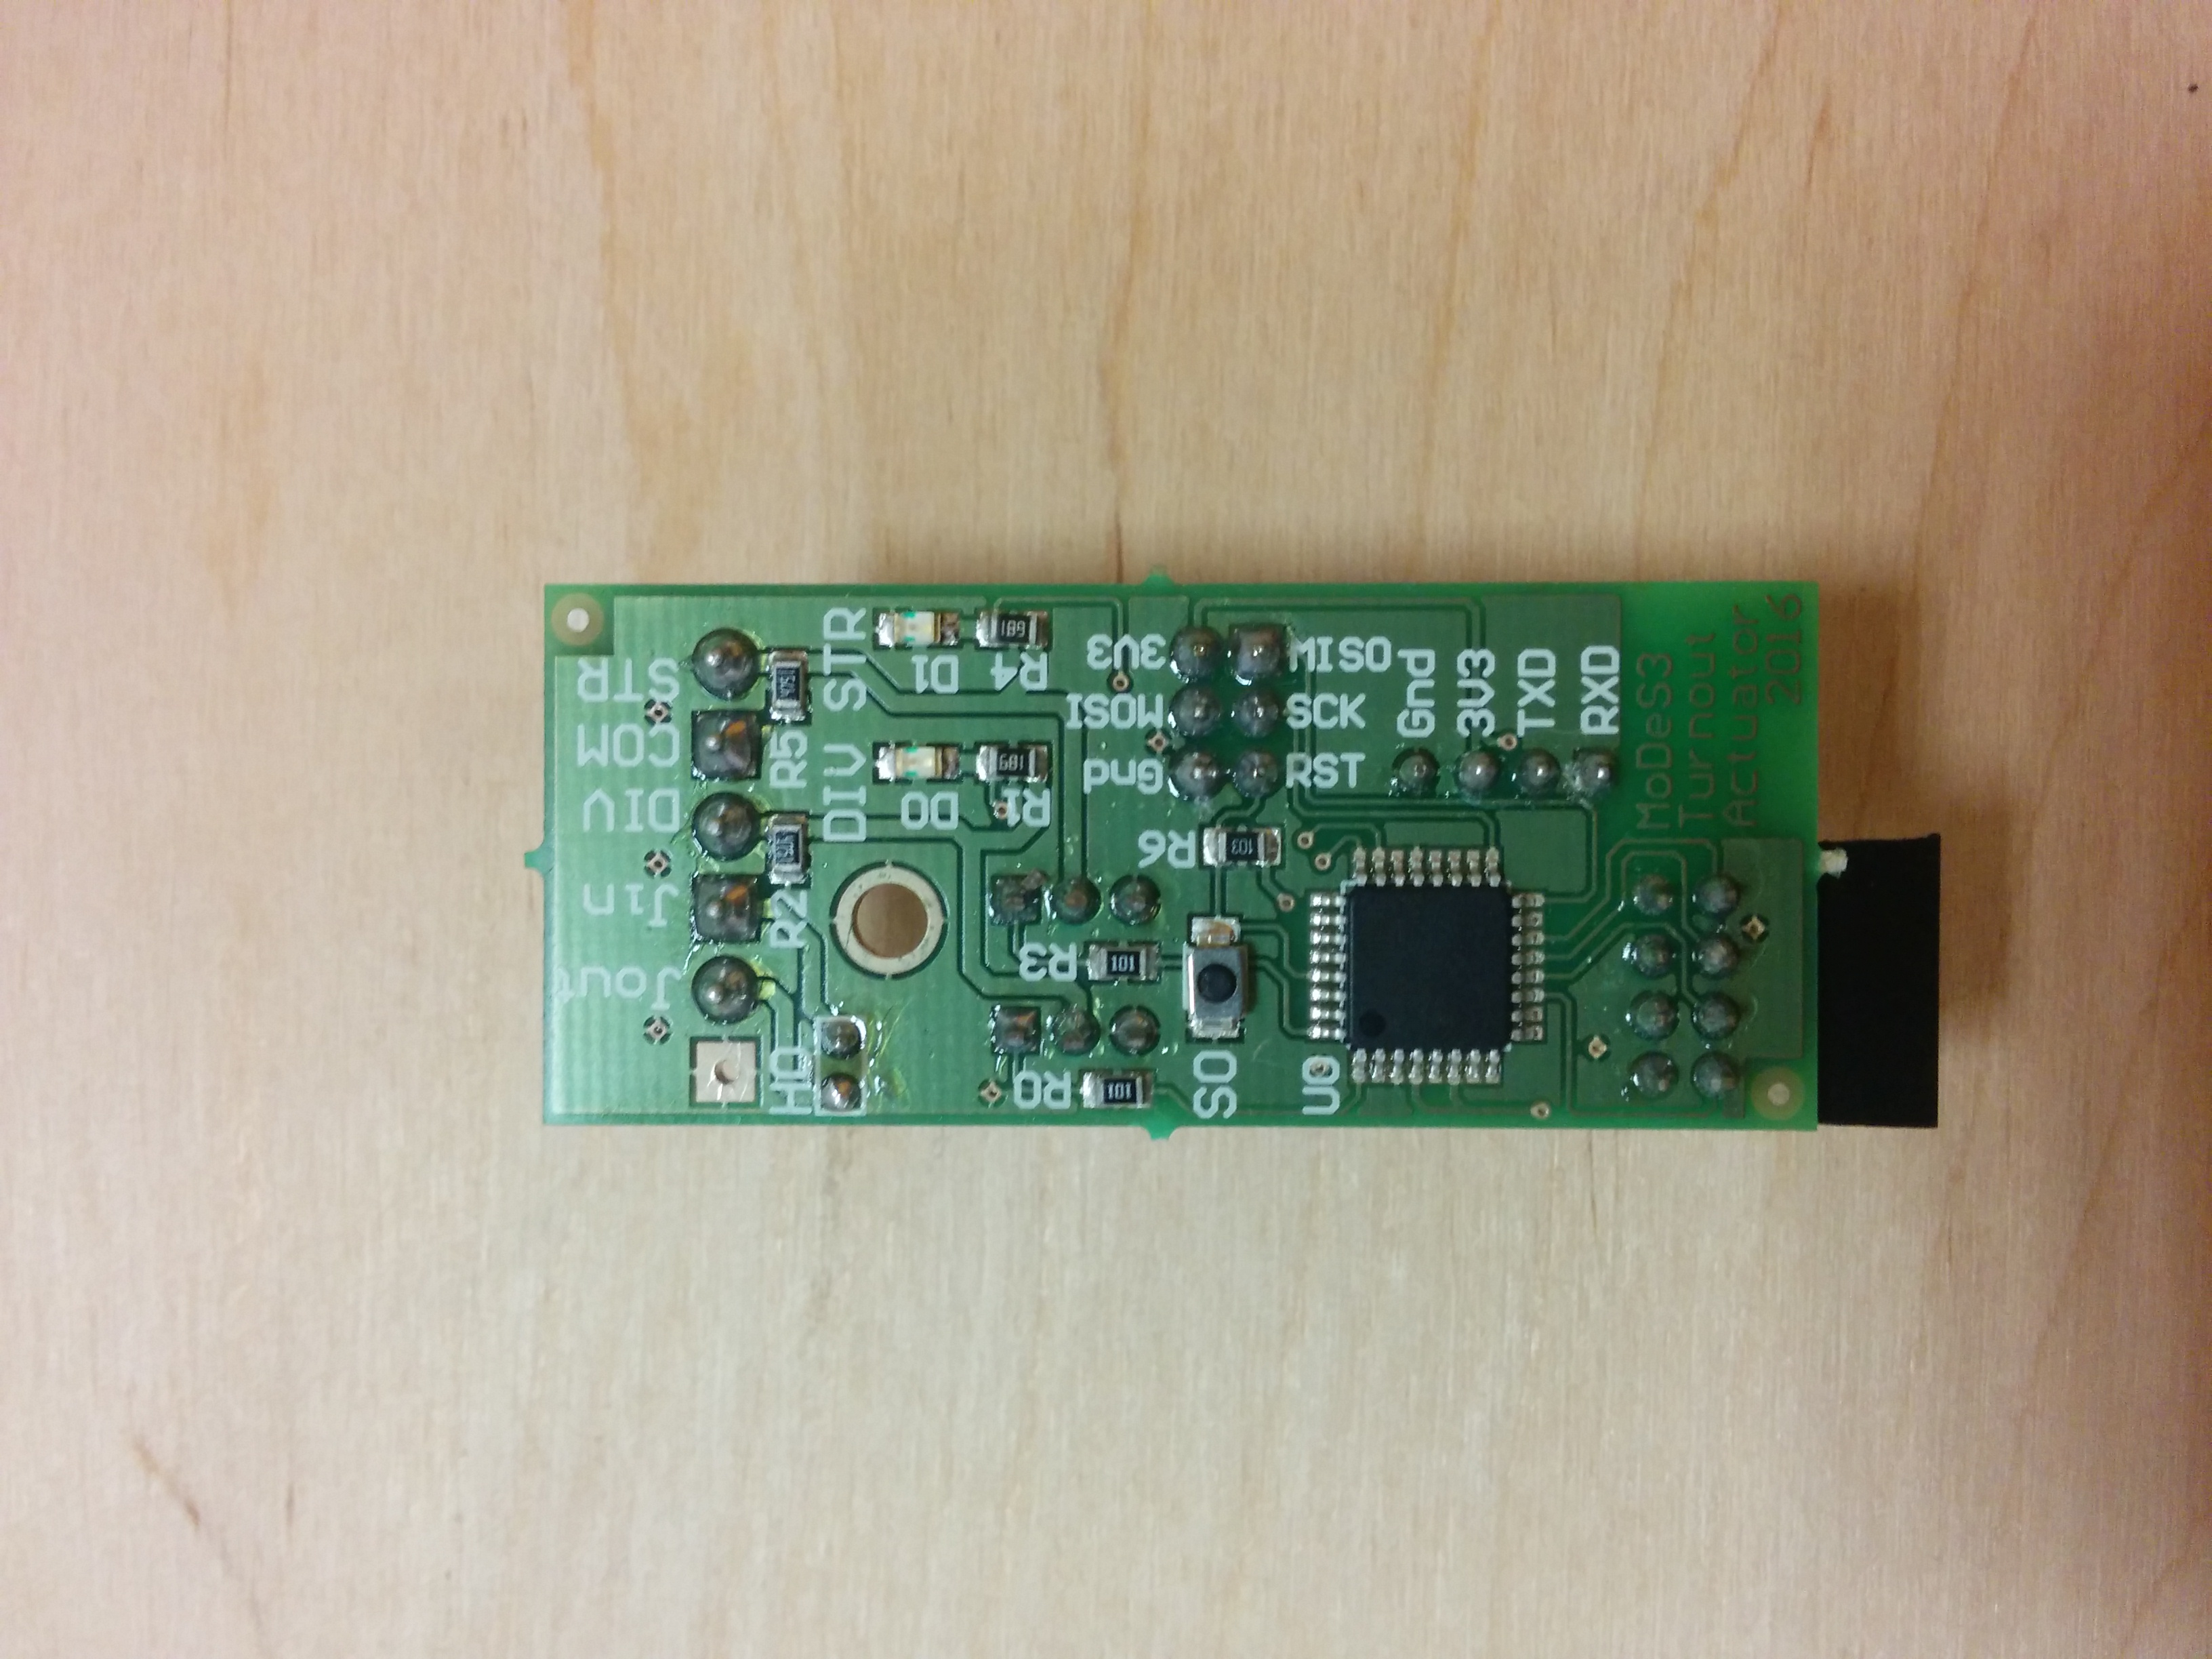
\includegraphics[width=100mm]{figures/modes3/turnout-top.jpg}
	\caption{Turnout actuator top view}
	\label{fig:turnoutTop}
\end{figure}

The concept behind this unit is based on the fact, that turnout mechanism is working as an wire between the common (COM) pole and an other pole (STR or DIV) when switched in one position, therefore we can sense its state.

The electronic characteristics of the BeagleBone unit could not satisfy the switching process electrically, thus we had to use a micro-controller (an Atmega328 MCU). Also, the state-sensing process is based on Analog to Digital Converters, which are also integrated into the MCU.

\textbf{Usage}
The MCU has 2 inputs and 2 outputs connected to the expander connector as shown in the table below.
\begin{center}
	\renewcommand{\arraystretch}{1.5}
	\begin{tabu} to 1.0\textwidth {X[c] X[c] X[c] X[c]}
		\toprule
		Pin 0                                  & Pin 1                                   & Pin 2                           & Pin 3                             \\ \midrule
		Turnout switching to Straight position & Turnout switching to Divergent position & Turnout state sensing (Straing) & Turnout state sensing (Divergent) \\
		INPUT for the MCU                      & INPUT for hte MCU                       & OUTPUT for the MCU              & OUTPUT for the MCU                \\ \bottomrule
	\end{tabu}
\end{center}


\section{Software components}
%\subsection{Deployment of software components}
\todo[inline]{Diagram of deployment}
\subsection{Occupancy detection elements} \label{section:OccupancyDetection}
\paragraph{Section Occupancy Query}
Responsible for debouncing the 32bit long occupancy vector with proper timing conditions regarding S88 protocol and forward this 32bit to OccupancyQuery through usb connection. Computed data contains the occupancy information for each track element (section or turnout) per one bit.
\paragraph{Occupancy Query}
In connection with the \textit{Section Occupancy Query} process the occupancy state for the whole track. Only if the state has changed, it sends occupancy change message to the mqtt topic with the track element id and new occupancy state.

\subsection{Track element control elements}
Deployed to the BBB hardware element.
\paragraph{GPIO}
Handle the GPIO pin changes and commands for each extension point of the BBB cape (see \ref{paragraph:BBBcape} section for details about BBB cape and expanders).
\paragraph{Physical Segment Controller}
For each segment there are two GPIO instance to serve the control mechanism of application and the PRU also, however there is no PRU control implemented.
\paragraph{Physical Turnout Controller}
For each turnout controller, there are four GPIO pins: two for control the turnout itself (straight and divergent direction), and other two to get info about the current state.
\paragraph{Track Element Controller}
Implementation of the platform-specific actuator code of disabling and enabling sections and setting turnout directions for the BeagleBone Black embedded units.

\subsection{Track control and inspection elements}
\paragraph{?XPressNet}
\paragraph{DashBoard}
Model railway track dashboard implementation. In Addition this component is instantiated only once, and up for the whole time while the track is in use. Consequently we can reach one common dashboard from the web and it contains the actual occupancy and track element status.
\paragraph{TouchBoard}
Dashboard for the model railway track, with focus on touchable elements, that can be controlled.
\paragraph{Safety Logic}
In the MODES$^3$ safety critical project we want to avoid the collision of model trains, therefore the safety logic software component detects these critical scenarios by Viatra Query patterns and act the necessary action (for example disable a section).

\subsection{Messaging elements}
Each software component share information about the railroad system through the messaging software element, which is based on protobuf messages and provides high-level designed API for this purpose. 

\subsection{Complementary elements}
\paragraph{Barrier} 
Sends open/close commands to the barrier over the network, depending on the occupancy of certain segments.
\paragraph{Leapmotion}
Software component for converting gestures into special movements for changing the speed of a specific train.

\section{Components by functional purpose}
\todo[inline]{figure + dietails about the functional / logical connections}